\documentclass[8pt]{beamer}

\mode<presentation>
{
  \usetheme{AnnArbor}
  \usecolortheme{beaver}
  \usefonttheme{default}
  \setbeamertemplate{caption}[numbered]
  \setbeamercovered{transparent}
  \usefonttheme[onlymath]{serif}
  \setbeamertemplate{itemize items}[default]
  \setbeamertemplate{navigation symbols}{\insertslidenavigationsymbol\insertframenavigationsymbol}
} 

\usepackage[english]{babel}
\usepackage[utf8x]{inputenc}
\usepackage{mathtools, xcolor, soul, amsfonts, appendixnumberbeamer, graphicx, tikz, caption}
\usepackage[makeroom]{cancel}
\graphicspath{ {images/} }

%\hypersetup{pdfpagemode=FullScreen}

\title[\scalebox{.68}{A Fast Algorithm for Learning a Ranking Function from Large-Scale Data Sets}]{A Fast Algorithm for Learning a Ranking Function\\from Large-Scale Data Sets}
\author[\scalebox{.8}{Dariush Hasanpoor}]{{\footnotesize IEEE Trans. On Pattern Analysis and Machine Intelligence, 2008}\\\vspace{3em}Dariush Hasanpoor}
\institute[]{Isfahan University Of Technology}
\date[Dec. 2015]{Dec. 2015}

\newcommand{\Xtri}{$\blacktriangleright$ }
\newcommand{\Ytri}{$\triangleright$ }
\newcommand{\itemXtri}{\item[\Xtri]}
\newcommand{\itemYtri}{\item[\Ytri]}
\renewcommand{\|}[1][.3em]{\hspace{#1}|\hspace{#1}}
\renewcommand{\,}[1][.3em]{,\hspace{#1}}
\newcommand\Wider[2][3em]{%
\makebox[\linewidth][c]{\begin{minipage}{\dimexpr\textwidth+#1\relax}\raggedright#2\end{minipage}}}
\newcommand*{\Scale}[2][4]{\scalebox{#1}{$#2$}}%
\DeclarePairedDelimiter\abs{\lvert}{\rvert}%

\makeatletter
    \let\oldabs\abs
    \def\abs{\@ifstar{\oldabs}{\oldabs*}}
\makeatother

\makeatletter
% The following two commands should only be given between frames

% Remove the equation counter from the list of counters that are reset after
% each overlay.
\def\donotresetequations{{%
    \let\@@elt\relax
    \def\@elt##1{%
        \expandafter\ifx\csname ##1\endcsname\c@equation%
        \else%
            \@@elt {##1}%
        \fi%
    }%
    \edef\beamer@overlaycounterresets{\beamer@overlaycounterresets}%
    \let\@elt\relax%
    \def\@@elt{\@elt}%
    \xdef\beamer@overlaycounterresets{\beamer@overlaycounterresets}%
}}

% Add the equation counter from the list of counters that are reset after
% each overlay.
\def\resetequations{\resetcounteronoverlays{equation}}
\makeatother

\newlength{\wideitemsep}
\setlength{\wideitemsep}{\itemsep}
\addtolength{\wideitemsep}{1em}
\let\olditem\item
\renewcommand{\item}{\setlength{\itemsep}{\wideitemsep}\olditem}

\DeclarePairedDelimiter{\ceil}{\lceil}{\rceil}

\definecolor{light-blue}{HTML}{66AFE9}
\definecolor{light-red}{HTML}{F77B7B}
\definecolor{light-green}{HTML}{87D13E}

\newcommand{\subitem}{\item[\Ytri]}
\newcommand{\Cpl}{\emph{Preference Learning} }
\newcommand{\pl}{\emph{preference learning} }
\newcommand{\Cp}{\emph{Preference} }
\newcommand{\p}{\emph{preference} }
\newcommand{\m}[1]{\mathcal{#1}}
\newcommand{\e}[1]{{\emph{#1}}}
\renewcommand{\,}{,\hspace{3pt}}
\renewcommand{\|}{\hspace{3pt}|\hspace{3pt}}
\newcommand{\argmax}{\arg\!\max}
\newcommand{\pr}[2]{{\partial #1 \over \partial #2}}
\newcommand{\erfc}{{\text{\textit{erfc}}}}
\renewcommand{\O}{\m{O}}
\newcommand{\eAcc}{$\epsilon$-Accurate }
\newcommand{\eacc}{$\epsilon$-accurate }

\begin{document}

\donotresetequations

\begin{frame}
  \titlepage
\end{frame}

\begin{frame}{Outline}
  \tableofcontents[hideallsubsections]
\end{frame}

\section{Introduction}
\frame{\tableofcontents[currentsection]}
\subsection{What is preference?}

\begin{frame}{What is preference?}

	\begin{block}{Definition}
	\Cpl refers to the task of learning to predict an order relation on a collection of objects (alternatives).
	\end{block}
    \begin{itemize}
    \item Preference information plays a key role in automated decision making and appears in various guises in AI researches:
        \begin{itemize}
        \subitem Qualitative decision theory
        \subitem Non-monotonic reasoning
        \subitem Constraint satisfaction
        \subitem Planning
        \end{itemize}
    \end{itemize}
\end{frame}

\subsection{Notations}

\begin{frame}{Notations}
	\begin{block}{\textbf{Definition:} \textit{Weak} \Cp}
	A weak \p relation  $\succeq$ on a set $\mathcal{A}$ is a reflexive and transitive binary relation.
	\end{block}
	\pause
	\begin{block}{\textbf{Definition:} \textit{Strict} \Cp}\center
	$a \succ b  \longleftrightarrow  (a \succeq b) \wedge (b \nsucceq a)$
	\end{block}
	\pause
    \begin{itemize}
    \item In agreement with preference semantics
        \begin{itemize}
        \item[] \vspace{1em}
            \begin{table}
	            \centering
	            \begin{tabular}{c|l}
	                \textit{Notation} & \textit{Interpretation} \\\hline\rule{0pt}{1.6em}
	                $a \succeq b$ & "alternative $a$ is at least as preferred as alternative $b$." \\\rule{0pt}{1.6em}
	                $a \succ b$ & "alternative $a$ is preferred over alternative $b$."\\
	            \end{tabular}
	        \end{table}
        \end{itemize}
    \end{itemize}
\end{frame}

\begin{frame}{Preference Structure}
	\begin{block}{\textbf{Definition:} \textit{Total Strict Order (Ranking)}}\footnotesize
	If $\mathcal{A}$ is a finite set of objects/alternatives $\{a_1,\ldots,a_m\}$ a ranking of $\mathcal{A}$ can be defined with a permutation $\tau$ of $\{1,\ldots,m\}$ which {\small $a_i \succ a_j \leftrightarrow \tau(i) < \tau(j)$}.
	\end{block}
	\pause
    \begin{itemize}
    \item $\mathcal{S}_m$ is a set of all permutation of $\tau$.
    \item The task of \textit{preference learner} is to search in $\mathcal{S}_m$ space which is \emph{learning to rank}.
    \end{itemize}
\end{frame}

\subsection{Types of Ranking}

\begin{frame}{Types of Ranking}
    \begin{itemize}
    \setlength\itemsep{1em}
    \item The tasks are categorized as three main problems:\\
        \begin{itemize}
        \setlength\itemsep{.5em}
        \itemXtri \textbf{Label ranking}
        \itemXtri \textbf{Object ranking}
        \itemXtri \textbf{Instance ranking}
        \end{itemize}
    \end{itemize}
\end{frame}

\begin{frame}{Types of Ranking}{Object Ranking}
    \begin{block}{\textbf{Task}}\small
    The task of this model is to find a preference ranking order among instances.
    \end{block}
    \pause
    \vskip .4cm
    \begin{itemize}
    \item[] \textbf{Given}
        \begin{itemize}
        \setlength\itemsep{.5em}
        \subitem A (potentially infinite) set X of objects (each object typically represented by a feature vector).
        \subitem A finite set of pairwise preferences $x_i \succ x_j$, $(x_i , x_j) \in \mathcal{X}\times\mathcal{X}$.
        \end{itemize}
    \pause
    \item[] \textbf{Find}
        \begin{itemize}
        \setlength\itemsep{1em}
        \subitem A ranking function that, given a set of objects $O \subset X$ as input, returns a permutation(ranking) of these objects.
        \end{itemize}
    \item<4-> In the training phase, preference learning algorithms have access to examples for which the order relation is \textbf{(partially)} known.
    \end{itemize}
\end{frame}

\subsection{Ranking Function}

\begin{frame}{Preference Relation and Ranking Function}
    \begin{itemize}
    \item Consider an instance space $\m{X}$ . For any $(x, y) \in \m{X} \times \m{X}$, we interpret the \emph{preference relation} $x \succeq y$, as “$x$ is at least as good as $y$.” We say that "$x$ is indifferent to $y$" $(x \sim y)$ if $x \succ y$ and $y \prec x$.
    \item One way of describing preference relations is by means of a ranking function.
    \item[] \begin{itemize}
        \subitem A function $f : \m{X} \rightarrow \mathbb{R}$  is a ranking/scoring function representing the preference relation $\succeq$ if:
        \begin{equation}\label{eq:ranking_func}
        \forall x, y \in \m{X},\hspace{1em} x \succeq y \Leftrightarrow f(x) \geq f(y)
        \end{equation}
        \subitem The ranking function $f$ provides a numerical score to the instances based on which the instances can be ordered.
        \subitem The function $f$ is not unique.
    \end{itemize}
    \end{itemize}
\end{frame}


\begin{frame}{Preference Relation and Ranking Function}
    \begin{itemize}
    \item The learnt \e{ranking function} should be \e{rational}, a \p relation $\succeq$ is called rational if  it satisfies the following two properties:
    \item[] \begin{itemize}
        \subitem \e{Completeness}. $\forall x, y, \in  \m{X}$, we have that $x \succeq y$ or $y \succeq x$.
        \subitem \e{Transitivity}. $\forall x, y, \in  \m{X}$, if $x \succeq y$ and $y \succeq z$, then $x \succeq z$.
    \end{itemize}
    \item A preference relation can be represented by a ranking function only if it is rational.
    \end{itemize}
    \vspace{3em}
    \begin{block}{}\centering
    The paper considers the learning of a preference relation as\\a problem of learning a rational ranking function.
    \end{block}
\end{frame}

\section{Learning a Ranking Function}
\frame{\tableofcontents[currentsection]}

\subsection{Problem Statement}
\begin{frame}{Problem Statement}
    \onslide{We are given training data $\m{A}$, a directed preference graph $\m{G} = (\m{V},\m{E})$ encoding the preference relations, and a function class $\m{F}$ from which we choose our ranking function $f$.}\vspace{1em}
    \begin{itemize}
    \item The training data $\m{A} = \cup_{j = 1}^S(\m{A}^j = \{x_i^j \in \mathbb{R}^d\}_{i = 1}^{m_j})$ contains $S$ classes(sets). Each class $\m{A}^j$ contains $m_j$ samples, and there are a total of $m = \sum_{j = 1}^S m_j$ samples in $\m{A}$.
    \item Each vertex of the directed order graph $\m{G} = (\m{V},\m{E})$ corresponds to a class $\m{A}^j$. The existence of a directed edge $\m{E}_{ij}$ from $\m{A}^i \rightarrow \m{A}^j$ means that all training samples in $\m{A}^j$ are preferred or ranked higher than any training sample in $A^i$, that is, $\forall(x_k^i \in \m{A}^i, x_l^j \in \m{A}^j),\hspace{0.5em}x_l^j \succ x_k^i$
    \end{itemize}
    \begin{figure}
    \centering
    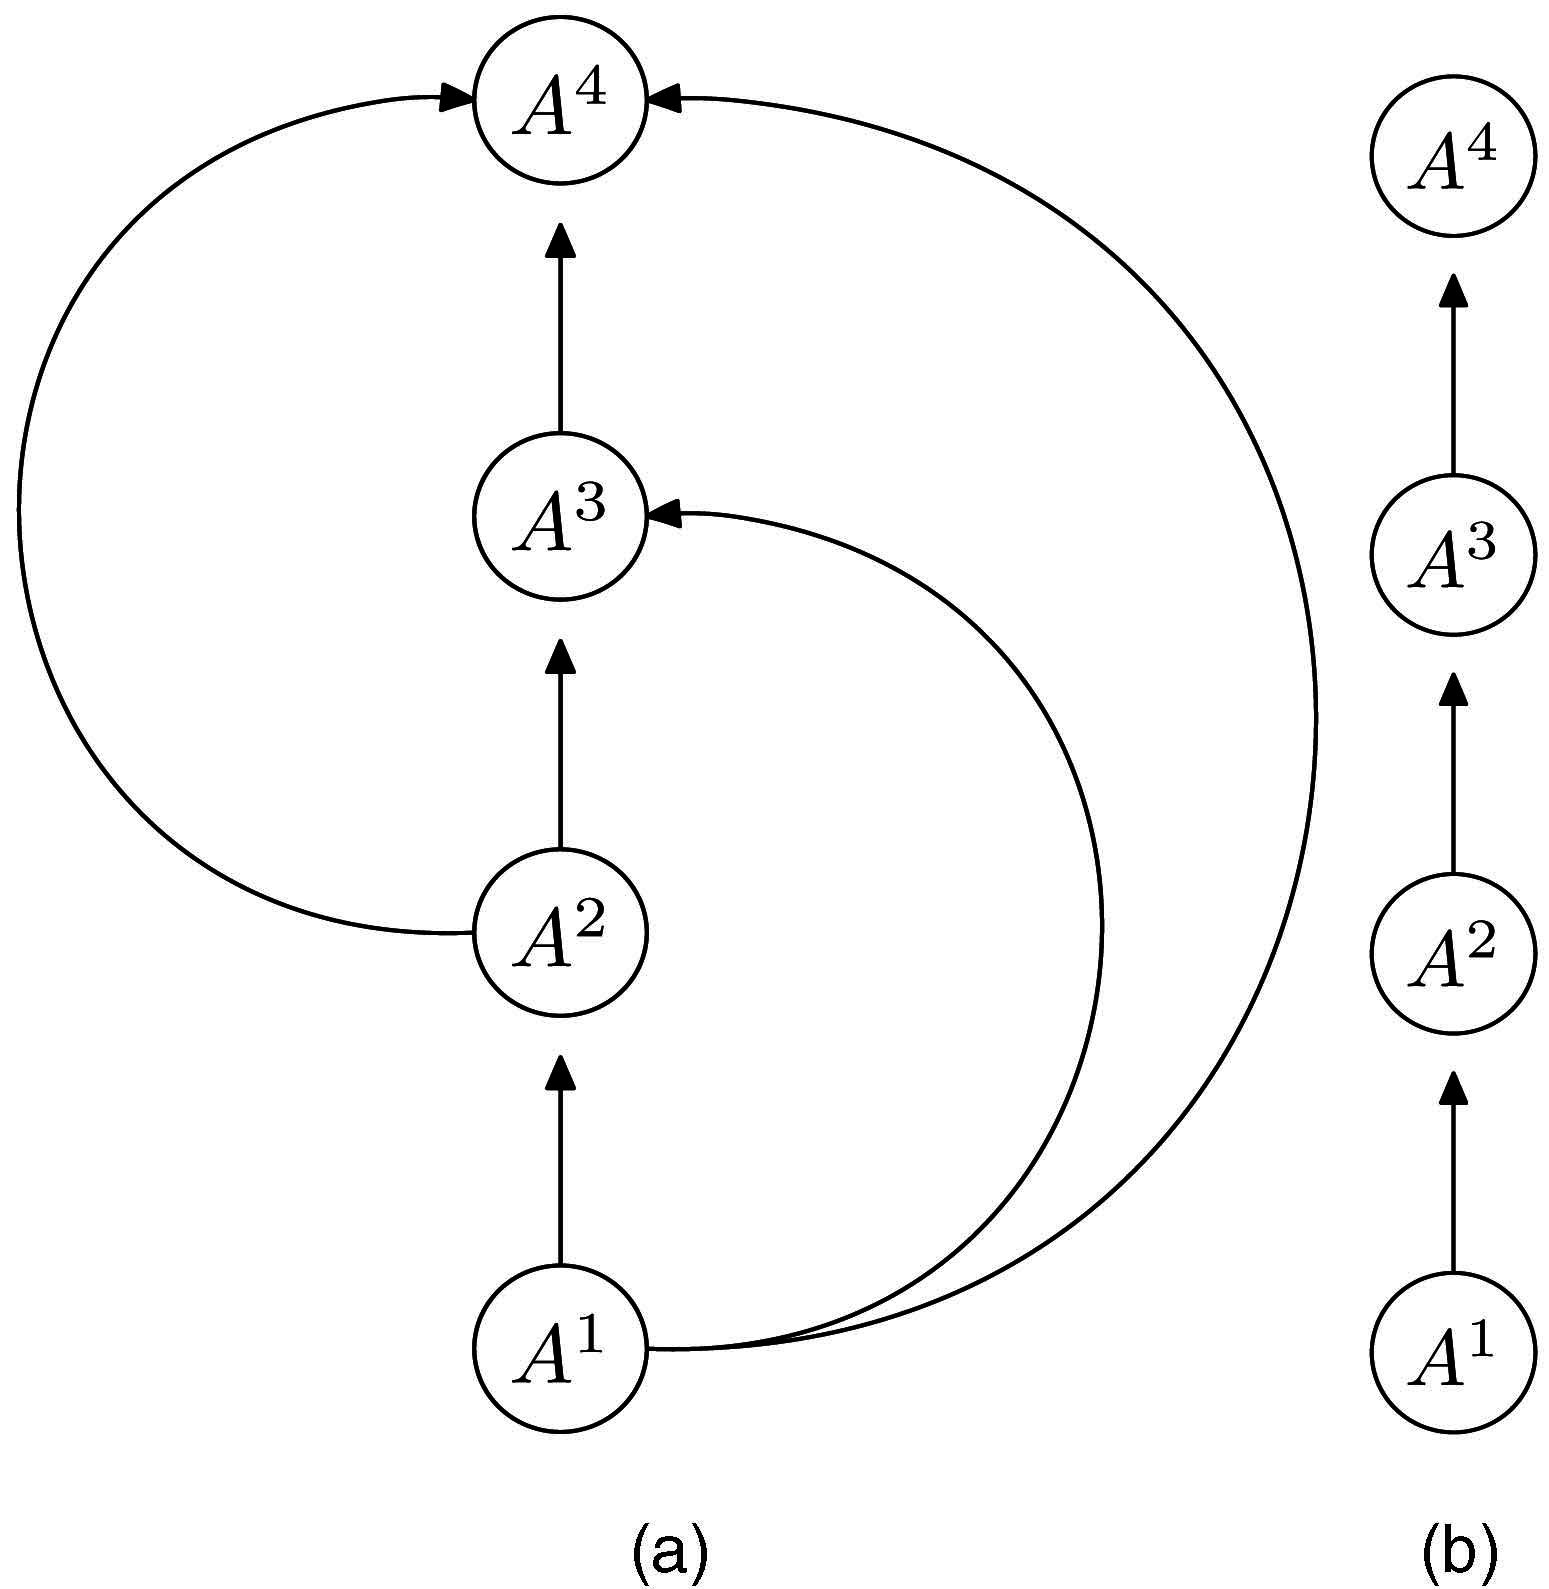
\includegraphics[width=.3\textwidth]{pr_graph}
    \caption[]{}
    \end{figure}
\end{frame}


\begin{frame}{Problem Statement}{Cont.}
    \begin{block}{The Goal}
    The goal is to learn a ranking function $f = \mathbb{R}^d \rightarrow \mathbb{R}$ such that $f(x_l^j) \succeq f(x_k^i)$ \e{for as mant pairs as possible} in the training data $\m{A}$ and also to perform well on unseen examples. 
    \end{block}
    \vspace{5em}
    \begin{itemize}
    \item The output $f(x_k)$ can be sorted to obtain a rank ordering for a set of test samples $\{x_k \in \mathbb{R}^d\}$.
    \end{itemize}
\end{frame}

\begin{frame}{Generalized Wilcoxon-Mann-Whitney Statistic}
    \begin{itemize}
    \item The Wilcoxon-Mann-Whitney(WMW) statistic is frequently used to assess the performance of a classifier because of its equivalence to the area under the Receiver Operating Characteristics (ROC) curve (AUC).
    \item  It is equal to the probability that a classifier assigns a higher value to the positive example than to the negative example, for a randomly
drawn pair of samples.
    \end{itemize}
    \begin{align}
    WMW(f, \m{A}, \m{G}) &= \frac{\sum_{\m{E}_{ij}}\sum_{k = 1}^{m_i}\sum_{l = 1}^{m_j} \textbf{1}_{f(x_l^j) \geq f(x_k^i)}}{\sum_{\m{E}_{ij}}\sum_{k = 1}^{m_i}\sum_{l = 1}^{m_j} 1}\label{eq:WMW_stat}\\
    \text{Where}\hspace{1em}\textbf{1}_{a \geq b} &= \begin{cases}
    1 & a \geq b\\
    0 & \text{otherwise}
    \end{cases}
    \end{align}
    \begin{itemize}
    \item The WMW statistic is thus an estimate of $Pr[f(x_1) \geq f(x_2)]$  for a randomly drawn pair of samples $(x_1, x_0)$ such that $x_1 \succeq x_0$.
    \item For a perfect ranking function, the WMW statistic is 1, and for a completely random assignment, the expected WMW statistic is 0.5.
    \end{itemize}
\end{frame}

\subsection{The MAP Estimator for Learning Ranking Functions}

\begin{frame}{The MAP Estimator for Learning Ranking Functions}
    \begin{itemize}
    \item The paper considered the family of linear ranking functions: $\m{F} = \{f_w\}$, where for any $x, w \in \mathbb{R}^d\,f_w(x) = w^Tx$.
    \end{itemize}
    \begin{block}{Objective:}
    Choose $w$ in order to maximize the generalize $WMW(f_w, \m{A}, \m{G})$.    
    \end{block}
    \begin{itemize}
    \item For computational efficiency, the paper maximizes a continues surrogate via the log likelihood:
    \item[] \begin{align}
    \m{L}(f_w, \m{A}, \m{G}) &= \log Pr[\text{correct ranking}|w]\nonumber\\
                             &\approx \prod_{\m{E}_{ij}}\prod_{k=1}^{m_i}\prod_{l=1}^{m_j}Pr[f_w(x_l^j) > f_w(x_k^i) | w]
                             \label{eq:continuous_surrogate_for_wmw}
    \end{align}.
    \item In \ref{eq:continuous_surrogate_for_wmw} we have assumed that every pair $(x_l^j,x_k^i)$ is drawn independently, whereas only the original samples are drawn independently.
    \end{itemize}
\end{frame}

\begin{frame}{The MAP Estimator for Learning Ranking Functions}{Cont.}
    \begin{itemize}
    \item[] \begin{align}
        Pr[f_w(x_l^j) > f_w(x_k^i) | w] &= \sigma[w^T(x_l^j - x_k^i)]\\
        \text{where\hspace{1em}} \sigma(z) &= {1 \over {1 + e^{-z}}}\nonumber
    \end{align}
    \item We will assumed a spherical Gaussian prior $p(w) = \m{N}(w|0, \lambda^{-1}\vec{I})$ on weights $w$.
    \item[] \begin{itemize}
        \item This encapsulates our prior belief that the individual weights in $w$ are independent and close to zero with a variance parameter $1 \over \lambda$.
    \end{itemize}
    \item The optimal \e{maximum a posteriori}(MAP) estimator is of the form:
    \item[] \begin{equation}
    \hat{w}_{\text{MAP}} = \argmax_{w} L(w)
    \end{equation}
    \item Where $L(w)$ is the penalized log likelihood:
    \item[] \begin{equation}
        L(w) = -{\lambda \over 2}\lVert w \rVert^2 + \sum_{\m{E}_{ij}}\sum_{k = 1}^{m_i}\sum_{l = 1}^{m_j} \log\sigma[w^T(x_l^j - x_k^i)]
        \label{eq:log_likelihood_L_w}
    \end{equation}
    \end{itemize}
\end{frame}

\begin{frame}{The MAP Estimator for Learning Ranking Functions}{Lower Bounding the WMW Statistic}
    \begin{itemize}
    \item Comparing the log-likelihood $L(w)$\ref{eq:log_likelihood_L_w} to the $WMW$ statistic (eq.\ref{eq:WMW_stat}), we can lower bounding the 0-1 indicator function in the $WMW$ statistic by a log-sigmoid function:
    \item[] \begin{equation}
    \textbf{1}_{z > 0} \geq 1 + ({ \log\sigma(z) \over \log_2})
    \end{equation}
    \item[] \begin{figure}
    \centering
    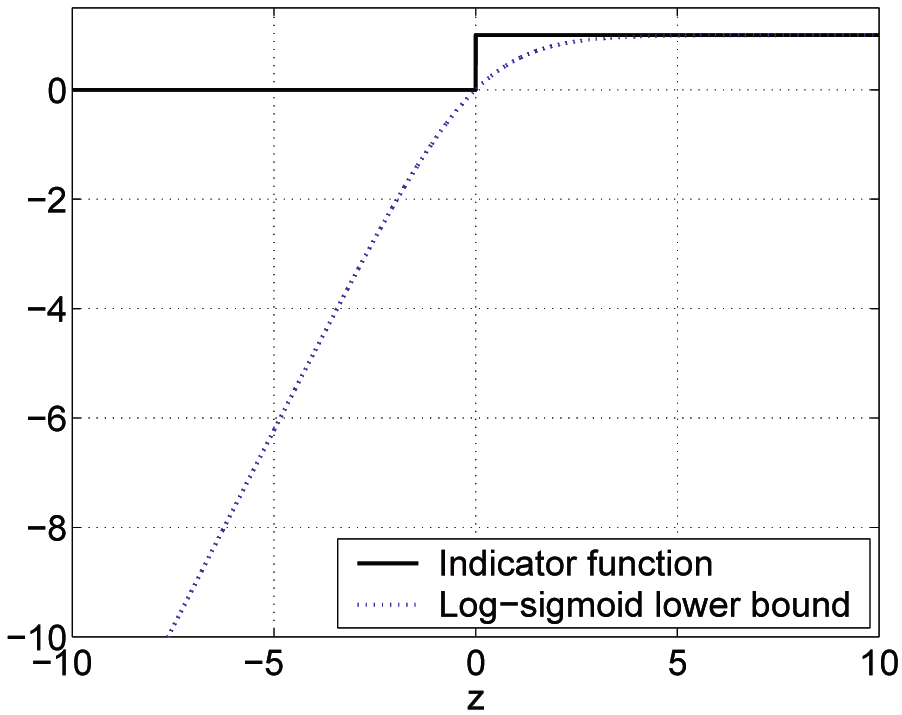
\includegraphics[width=.3\textwidth]{wmw_01_indic_bound}
    \caption[]{}
    \end{figure}
    \end{itemize}
    \begin{block}{Therefore:}\centering
    Maximizing the penalized log likelihood is equivalent to maximizing a lower bound on the $WMW$ statistic.
    \end{block}
\end{frame}

\subsection{The Optimization Algorithm}

\begin{frame}{The Optimization Algorithm}
    \begin{itemize}
    \item \textbf{Objective:} Maximizing the penalized log likelihood, with respect to $w$.
    \item We use the Polak-Ribi\`{e}re variant of nonlinear conjugate gradients(CG) algorithm.
    \item[] \begin{itemize}
        \subitem The CG method only needs the gradient $g(w)$ and does not require evaluation of $L(w)$.
        \subitem It also avoids the need for computing the second derivatives(Hessian matrix).
    \end{itemize}
    \item[] \begin{align}
        L(w) &= -{\lambda \over 2}\lVert w \rVert^2 + \sum_{\m{E}_{ij}}\sum_{k = 1}^{m_i}\sum_{l = 1}^{m_j} \log\sigma[w^T(x_l^j - x_k^i)]\nonumber\\
        g(w_i) = \pr{L(w)}{w_i} &= -\lambda w_i - \sum_{\m{E}_{ij}}\sum_{k = 1}^{m_i}\sum_{l = 1}^{m_j} (x_l^i - x_k^j)\sigma[w^T(x_l^j - x_k^i)]\label{eq:gradient_func}
    \end{align}
    \end{itemize}
\end{frame}

\begin{frame}{The Optimization Algorithm}{What cost us so much!?}
    \begin{itemize}
    \item[] \begin{equation}
    g(w) = -\lambda w - \sum_{\m{E}_{ij}}\sum_{k = 1}^{m_i}\sum_{l = 1}^{m_j} (x_l^i - x_k^j)\sigma[w^T(x_l^j - x_k^i)]
    \end{equation}
    \item The evaluation of the penalized log likelihood or its gradient requires $\m{M}^2 = \sum_{\m{E}_{ij}}m_im_j$ operations --- $\O(\m{M}^2)$.
    \item The main contribution of the paper is an extremely fast method to compute the gradient \e{approximately}.
    \end{itemize}
\end{frame}

\begin{frame}{The Optimization Algorithm}{Gradient Approximation Using the Error Function}
    \begin{itemize}
    \item We shall rely on the approximation:
    \item[] \begin{equation}
    \sigma(z) \approx 1 - {1 \over 2} \erfc\Big({\sqrt{3} z \over \sqrt{2} \pi}\Big)
    \end{equation}
    \item[] \begin{figure}
    \centering
    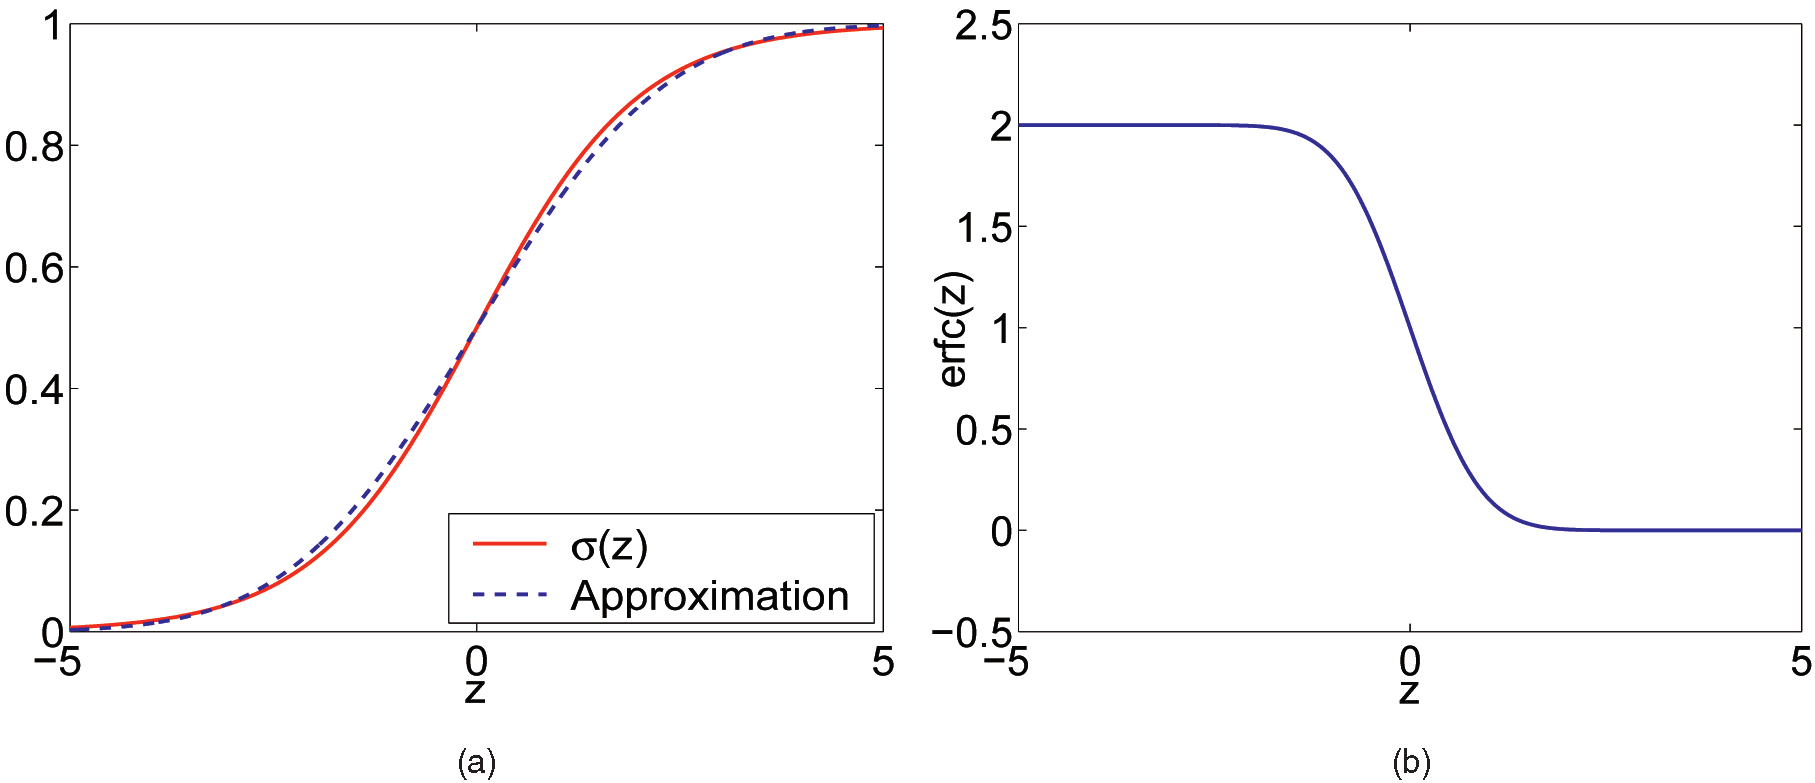
\includegraphics[width=.8\textwidth]{sigma_approx}
    \caption{(a) Approximation of the sigmoid function $\sigma(z) \approx 1 - {1 \over 2} \erfc\Big({\sqrt{3} z \over \sqrt{2} \pi}\Big)$. (b) The erfc function.}
    \end{figure}
    \end{itemize}
\end{frame}


\begin{frame}{The Optimization Algorithm}{Gradient Approximation Using the Error Function}
    \begin{itemize}
    \item Where the \e{erfc} defined as:
    \item[] \begin{equation}
    \erfc(z) = {2 \over \sqrt{\pi}}\int_z^\infty e^{-t^2}dt
    \end{equation}
    \item considering the $\sigma(z) \approx 1 - {1 \over 2} \erfc\Big({\sqrt{3} z \over \sqrt{2} \pi}\Big)$ the eq.\ref{eq:gradient_func} can be approximated as:
    \item[] \begin{align}
    g(w) &= -\lambda w - \sum_{\m{E}_{ij}}\sum_{k = 1}^{m_i}\sum_{l = 1}^{m_j} (x_l^i - x_k^j)\sigma[w^T(x_l^j - x_k^i)]\nonumber\\
    &\approx -\lambda w - \sum_{\m{E}_{ij}}\sum_{k = 1}^{m_i}\sum_{l = 1}^{m_j} (x_l^i - x_k^j)\Bigg[1 - {1 \over 2} \erfc\Big({\sqrt{3} w^T(x_l^j - x_k^i) \over \sqrt{2} \pi}\Big)\Bigg]
    \end{align}
    \end{itemize}
\end{frame}

\begin{frame}{The Optimization Algorithm}{Quadratic Complexity of Gradient Evaluation}
    \begin{block}{To summarize variables}
    \begin{itemize}
    \item We have $S$ classes with $m_i$ training instances in the $i$th class.
    \item Hence, we have a total of $m = \sum_{i = 1}^Sm_i$ training examples in $d$ dimensions.
    \item $\abs{\m{E}}$ is the number for edges in the preference graph.
    \item $\m{M}^2 = \sum_{\m{E}_{ij}} m_im_j$ is the total number of pairwise preference relations.
    \item \textbf{Definition:} $\forall x \in \m{A}\, z = {\sqrt{3}w^Tx \over \sqrt{2}\pi}$ is scalar and for a given $w$ can be computed in $\O(dm)$ operations for the entire training set.
    \end{itemize}
    \end{block}
\end{frame}

\begin{frame}{The Optimization Algorithm}{Quadratic Complexity of Gradient Evaluation(Cont.)}
    \begin{itemize}
    \item We will isolate the key computational primitive contributing to the quadratic complexity in the gradient computation.
    \item[] \begin{align}
    g(w) &\approx -\lambda w - \sum_{\m{E}_{ij}}\sum_{k = 1}^{m_i}\sum_{l = 1}^{m_j} (x_l^i - x_k^j)\Bigg[1 - {1 \over 2} \erfc\Big({\sqrt{3} w^T(x_l^j - x_k^i) \over \sqrt{2} \pi}\Big)\Bigg]\nonumber\\
    &= -\lambda w -\Delta_1 + {1 \over 2}\Delta_2 - {1 \over 2}\Delta_3
    \end{align}
    \item[] Where the \e{vectors} $\Delta_1\, \Delta_2 \text{ and } \Delta_3$ are defined as follows:
    \item[] \vspace{-1.5em}\begin{align}
    \begin{split}
    \Delta_1 &= \sum_{\m{E}_{ij}}\sum_{k = 1}^{m_i}\sum_{l = 1}^{m_j} (x_k^i - x_l^j)\\
    \Delta_2 &= \sum_{\m{E}_{ij}}\sum_{k = 1}^{m_i}\sum_{l = 1}^{m_j} x_k^i\erfc(z_k^i - z_l^j)\\
    \Delta_3 &= \sum_{\m{E}_{ij}}\sum_{k = 1}^{m_i}\sum_{l = 1}^{m_j} x_l^j\erfc(z_k^i - z_l^j)
    \end{split}
    \end{align}
    \end{itemize}
\end{frame}

\begin{frame}{The Optimization Algorithm}{Quadratic Complexity of Gradient Evaluation(Cont.)}
    \begin{itemize}
    \item The vector $\Delta_1 = \sum_{\m{E}_{ij}}\sum_{k = 1}^{m_i}\sum_{l = 1}^{m_j} (x_k^i - x_l^j)$ is independent of $w$ and can be written as follows: \[\Delta_1 = \sum_{\m{E}_{ij}} m_im_j(x_{\text{mean}}^i - x_{\text{mean}}^j)\]
    where $x_{\text{mean}}^i = {1 \over m_i} \sum_{k = 1}^{m_i}x_k^i$ is the mean of all the training instances in the $i$th class.
    \item $\Delta_1$ can be precomputed in $\O(\abs{\m{E}}d + dm)$ operations.
    \end{itemize}
\end{frame}

\begin{frame}{The Optimization Algorithm}{Quadratic Complexity of Gradient Evaluation(Cont.)}
    \begin{itemize}
    \item The other two terms $\Delta_2 $ and $\Delta_3$ can be written as follows:
    \item[] \begin{equation}
    \Delta_2 = \sum_{\m{E}_{ij}}\sum_{k = 1}^{m_i} x_k^iE_{-}^j(z_k^i)\hspace{2em}
    \Delta_3 = \sum_{\m{E}_{ij}}\sum_{l = 1}^{m_j} x_l^jE_{+}^i(-z_l^j)
    \end{equation}     
    where
    \begin{align}
    \begin{split}
    E_{-}^j(y) &= \sum_{l = 1}^{m_j}\erfc(y - z_l^j)\\
    E_{+}^i(y) &= \sum_{k = 1}^{m_i}\erfc(y + z_k^i)
    \end{split}
    \end{align}
    \item Each of $\Delta_2 $ and $\Delta_3$ can be computed in $\O(dSm + \m{M}^2)$ operations.
    \end{itemize}
\end{frame}

\begin{frame}{The Optimization Algorithm}{Quadratic Complexity of Gradient Evaluation(Cont.)}
    \begin{itemize}
    \item The core computational primitive contributing to the $\O(\m{M}^2)$ cost is the summation of \erfc\  functions.
    \item The paper showed that the sum can be computed in linear $\O(m_i + m_j)$ time, at the expense of reduced accuracy, which however can be arbitrary. As the result the $\Delta_2 $ and $\Delta_3$ can be computed in linear $\O(dSm + (S-1)m)$ time.
    \end{itemize}
\end{frame}

\subsection{Fast Weighted Summation Of erfc Functions}

\begin{frame}{Fast Weighted Summation Of erfc Functions}
    \begin{itemize}
    \item In general, $E_{-}^j(y)$ and $E_{+}^i(y)$  can be written as the weighted summation of N \erfc functions centred at $z_i \in R$ with weights $q_i \in R$.
    \begin{equation}
    E(y) = \sum_{i = 1}^Nq_i\erfc(y - z_i)\label{eq:e_y}
    \end{equation}
    \item Direct computation of eq.\ref{eq:e_y} at $M$ points $\{y_j \in \mathbb{R}\}_{j = 1}^M$ is $\O(MN)$.
    \item we will derive an \eacc approximation algorithm to compute this in $\O(M + N)$ time.
    \end{itemize}
\end{frame}

\begin{frame}{Fast Weighted Summation Of erfc Functions}{\eAcc Approximation}
    \begin{itemize}
    \item For any given $\epsilon > 0$, we define $\hat{E}$ to be an \eacc approximation to $E$ if the maximum absolute error relative to the total weight $Q_{\text{abs}} = \sum_{i = 1}^N \abs{q_i}$ is upper bounded by a specified $\epsilon$, that is:
    \begin{equation}
    \max_{y_i}\Bigg[{\abs{\hat{E}(y_j) - E(y_j)} \over Q_{\text{abs}}}\Bigg] \leq \epsilon
    \end{equation}
    \item The constant in $\O(M + N)$ for the algorithm depends on the desired accuracy $\epsilon$, which however can be \e{arbitrary}.
    \item The fast algorithm is based on using an infinite series expansion for the erfc function and retaining only the first few terms (whose contribution is at the desired accuracy).
    \end{itemize}
\end{frame}

\begin{frame}{Fast Weighted Summation Of erfc Functions}{Series Expansion for \erfc Function}
    \begin{itemize}
    \item The paper uses the following truncated Fourier series representation:
    \begin{align}
    \erfc(z) &= 1 - {4 \over \pi}\sum_{\substack{n=1 \\ \text{n odd}}}^{2p-1}{e^{-n^2h^2} \over n}\sin(2nhz) + error(z)\label{eq:erfc_f_series_approx}\\
    \abs{error(z)} &< \abs{{4 \over \pi}\sum_{\substack{n=2p+1 \\ \text{n odd}}}^{\infty}{e^{-n^2h^2} \over n}\sin(2nhz)} + \erfc({\pi \over 2h} - \abs{z})\label{eq:erfc_f_series_approx_error_bound_0}
    \end{align}
    where $p$ is known as the \e{truncation number} and $h$ is a real number related to the sampling interval.
    \item The series is derived by applying a \e{Chernoff bound} to an approximate \e{Fourier series expansion} of a periodic square waveform.
    \item This series converges rapidly, especially as $z \rightarrow 0$.
    \end{itemize}
\end{frame}

\begin{frame}{Fast Weighted Summation Of erfc Functions}{Series Expansion for \erfc Function(Cont.)}
    \begin{itemize}
    \item Figure \ref{fig:erfc_trunc_f_series} shows the maximum absolute error between the actual value of \erfc and the truncated series representation as a function of $p$.
    \begin{figure}
    \centering
    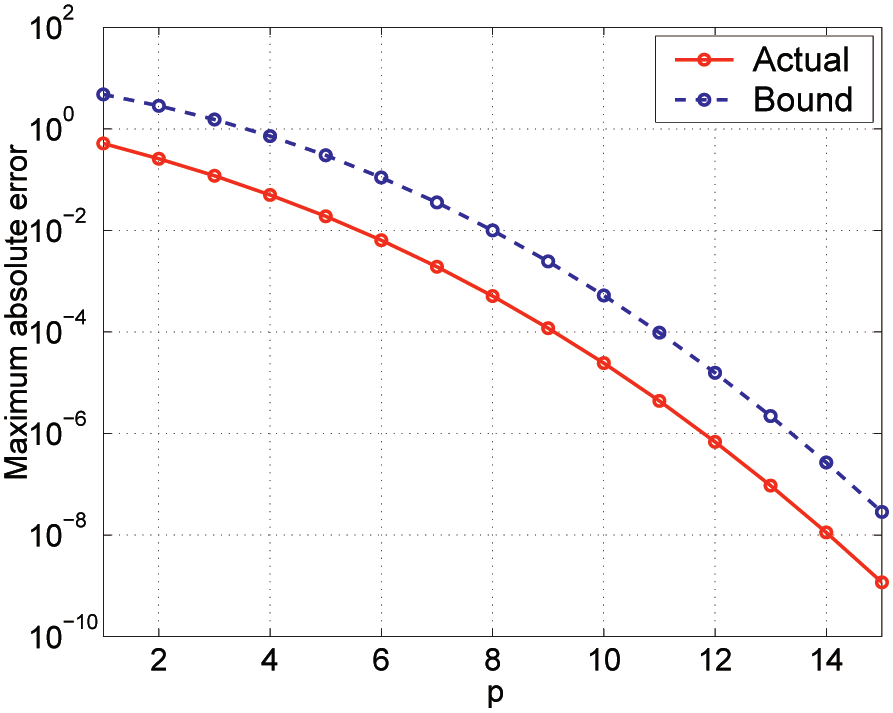
\includegraphics[width=.5\textwidth]{erfc_trunc_f_series}
    \caption[]{\centering The maximum absolute error between the actual value of \erfc and the truncated series representation eq.\ref{eq:erfc_f_series_approx} as a function of the truncation
number p for any $z \in [-4,4]$. The error bound eq.\ref{eq:erfc_f_series_approx_error_bound_1} is also shown as adotted line}\label{fig:erfc_trunc_f_series}
    \end{figure}
    \end{itemize}
\end{frame}

\begin{frame}{Fast Weighted Summation Of erfc Functions}{Error Bound}
    \only<-2>{\begin{itemize}
    \item We will have to choose $p$ and $h$ such that the error is less than the desired $\epsilon$. For this purpose, we further bound the first term in eq. \ref{eq:erfc_f_series_approx_error_bound_0} as follows:
    \end{itemize}}
    \only<1>{
    \begin{equation*}
        \abs{error(z)} < \abs{{4 \over \pi}\sum_{\substack{n=2p+1 \\ \text{n odd}}}^{\infty}{e^{-n^2h^2} \over n}\sin(2nhz)} + \erfc({\pi \over 2h} - \abs{z})
    \end{equation*}
    }    
    \only<2>{\tiny\begin{align*}
    &\abs{{4 \over \pi}\sum_{n=2p+1}^{\infty}{e^{-n^2h^2} \over n}\sin(2nhx)}\\
    &\leq {4 \over \pi}\sum_{n=2p+1}^{\infty}{e^{-n^2h^2} \over n}\abs{\sin(2nhx)}\\
    \xRightarrow{\abs{\sin(2nhx)} \leq 1} &\leq {4 \over \pi}\sum_{n=2p+1}^{\infty}{e^{-n^2h^2} \over n}\\
    \xRightarrow{{1 \over n} \leq 1} &< {4 \over \pi}\sum_{n=2p+1}^{\infty}e^{-n^2h^2}\\
    \xRightarrow{\sum \rightarrow \int} &< {4 \over \pi}\int_{2p+1}^{\infty}e^{-x^2h^2}dx\\
    &< {2 \over \sqrt{\pi}h}\Bigg[{2 \over \sqrt{\pi}} \int_{(2p+1)h}^{\infty} e^{-t^2}dt\Bigg]\\
    &= {2 \over \sqrt{\pi}h}\erfc((2p+1)h)
    \end{align*}}%
    \only<3>{
    \begin{itemize}
    \item Hence, the final error bound is of the form:
    \end{itemize}
    \begin{equation}
    \abs{error(z)} < {2 \over \sqrt{\pi}h}\erfc((2p+1)h) + \erfc({\pi \over 2h} - \abs{z})
    \end{equation}
    }
\end{frame}

\subsection{Fast Summation Algorithm}
\begin{frame}{Fast Weighted Summation Of erfc Functions}{Fast Summation Algorithm}
    \begin{itemize}
    \only<-1>{\item We now derive a fast algorithm to compute $E(y)$ based on the series eq.\ref{eq:erfc_f_series_approx}
    \begin{align}
    E(y) &= \sum_{i = 1}{N} q_i\erfc(y - z_i)\nonumber\\
    & = \sum_{i = 1}{N} q_i\Bigg[1 - {4 \over \pi}\sum_{\substack{n = 1\\\text{n odd}}}^{2p-1}{e^{-n^2h^2} \over n}\sin\{2nh(y - z_i)\} + error\Bigg]
    \end{align}}
    \only<-2>{
    \item Ignoring the error term for the time being, the sum $E(y)$ can be approximated as:
    \begin{equation}
    \hat{E}(y) = Q - {4 \over \pi}\sum_{i = 1}^{N}q_i\sum_{\substack{n = 1\\\text{n odd}}}^{2p-1}{e^{-n^2h^2} \over n}\sin\{2nh(y - z_i)\}
    \end{equation}
    where $Q = \sum_{i = 1}^{N}q_i$.
    \item The terms $y$ and $z_i$ are entangled in the argument of the $\sin$ function, leading to a quadratic complexity.}
    \only<2>{\item The crux of the algorithm is to separate them using the trigonometric identity:
    \begin{align}
    \begin{split}
    &\sin\{2nh(y - z_i)\}\\
    & = \sin\{2nh(y - z_*) - 2nh(z_i - z_*)\}\\
    & = \sin\{2nh(y - z_*)\}\cos\{2nh(z_i - z_*)\} - \cos\{2nh(y - z_*)\}\sin\{2nh(z_i - z_*)\}
    \end{split}
    \end{align}}
    \only<3>{
    \item[]
    \begin{align}
    \hat{E}(y) = Q - {4 \over \pi}\sum_{i = 1}^{N}q_i\sum_{\substack{n = 1\\\text{n odd}}}^{2p-1}&{e^{-n^2h^2} \over n}*\nonumber\\
    &\Bigg[\sin\{2nh(y - z_*)\}\cos\{2nh(z_i - z_*)\} -\nonumber\\
    &\cos\{2nh(y - z_*)\}\sin\{2nh(z_i - z_*)\}\Bigg]
    \end{align}
    \item Note that we have shifted all the points by $z_*$.
    \item[] \begin{itemize}
    \subitem The reason for this is that we cluster the points and use the series representation around the different cluster centres.
    \end{itemize}}
    \only<4>{
    \item Substituting the separated representation and exchanging the order of summation and regrouping the terms, we have the following expression:
    \begin{align}
    \begin{split}
    \hat{E}(y) = Q &- {4 \over \pi}\sum_{\substack{n = 1\\\text{n odd}}}^{2p-1}A_n\sin\{2nh(y - z_*)\}\\
    &+ {4 \over \pi}\sum_{\substack{n = 1\\\text{n odd}}}^{2p-1}B_n\cos\{2nh(y - z_*)\}
    \end{split}
    \end{align}
    \begin{align}
    \begin{split}
    A_n &= {e^{-n^2h^2} \over n}\sum_{i = 1}^{N}q_i\cos\{2nh(z_i - z_*)\}\\
    B_n &= {e^{-n^2h^2} \over n}\sum_{i = 1}^{N}q_i\sin\{2nh(z_i - z_*)\}
    \end{split}
    \end{align}
    }
    \end{itemize}
\end{frame}

\begin{frame}{Fast Weighted Summation Of erfc Functions}{Computational and Space Complexity}
    \begin{itemize}
    \item The coefficients $\{A_n, B_n\}$ do not depend on $y$. Hence, each of $A_n$ and $B_n$ can be evaluated separately in $\O(N)$ times.
    \item Since there are $p$ such coefficients the total complexity to computed $A$ and $B$ is $\O(pN)$.
    \item The term $Q = \sum_{i = 1}^Nq_i$ can also be pre-computed in $\O(N)$ time.
    \item Once $A\, B$ and $Q$ have been \e{pre-computed}, evaluation of $\hat{E}(y)$ requires $\O(p)$ operations. Evaluating at $M$ points is $\O(pM)$.
    \item Therefor, the computational complexity has reduced from the quadratic $\O(NM)$ to the linear $\O(p(N+M))$.
    \item The space needed to store the points and the coefficients $A$ and $B$, is $\O(N + M + p)$.
    \end{itemize}
\end{frame}

\begin{frame}{Fast Weighted Summation Of erfc Functions}{Direct Inclusion and Exclusion of Far Away Points}
    \only<-2>{
    \begin{equation*}
    \abs{error(z)} < {2 \over \sqrt{\pi}h}\erfc((2p+1)h) + \erfc({\pi \over 2h} - \abs{z})
    \end{equation*}
    }    
    \begin{itemize}
    \item  For a fixed $p$ and $h$ as $\abs{z}$ increases the error increases. Therefor as $\abs{z}$ increases, $h$ should decreases, consequently, the series converges slower leading to a large truncation number $p$.
    \item Note that $s = (y - z_i) \in [-\infty, \infty]$. the truncation number $p$ required to approximate $\erfc(s) \rightarrow 2$ as $s \rightarrow -\infty$ and $\erfc(s) \rightarrow 0$ as $s \rightarrow \infty$ very quickly.
    \only<1>{
    \begin{figure}
    \centering
    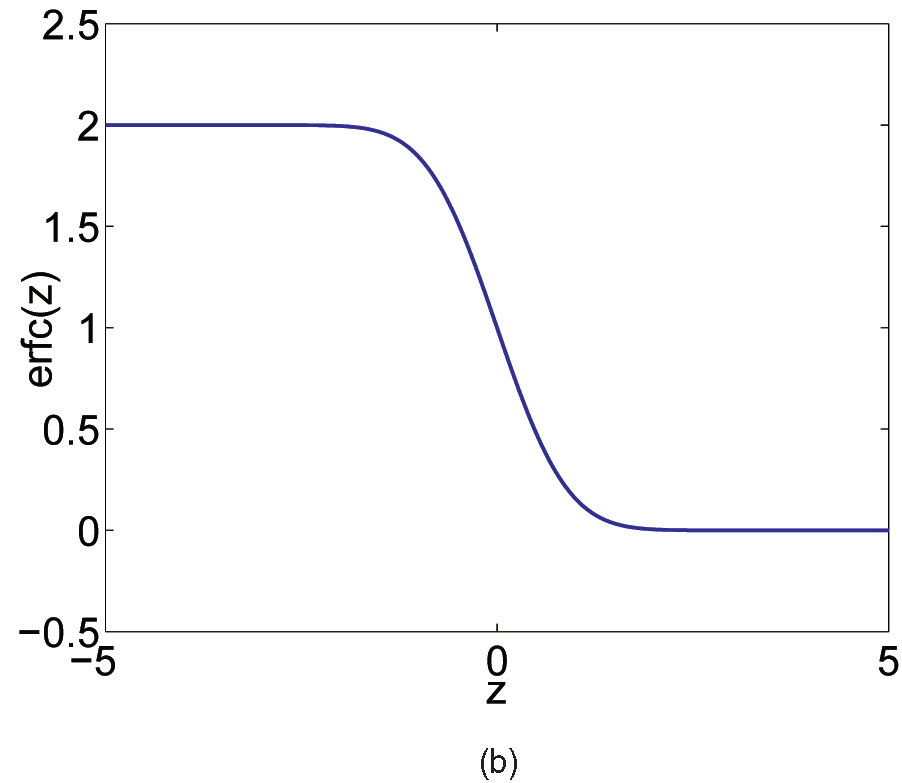
\includegraphics[width=.3\textwidth]{erfc}
    \end{figure}
    }
    \only<2>{
    \item We only want an accuracy of $\epsilon$, we can use the approximation:
    \begin{equation}
    \erfc(c) \approx \begin{cases}
    2 & s < -r\\
    \text{p-truncated series} & -r \leq s \leq r\\
    0 & s > r
    \end{cases}
    \end{equation}
    The bound $r$ and the truncation number $p$ have to be chosen such that for any $s$, the error is always less than $\epsilon$.
    }
    \end{itemize}
\end{frame}

%\begin{frame}{Fast Weighted Summation Of erfc Functions}{Space Subdivision}
%    \begin{itemize}
%    \only<1>{
%    \item We uniformly subdivide the domain into $K$ intervals of length $2r_x$.
%    \item The $N$ source points are assigned into $K$ clusters $S_k$, for $k = 1,\ldots,K$ with $c_k$ being the center of each cluster.
%    \item The aggregated coefficients are computed for each cluster, and the total contribution from all the influential clusters is summed up.
%    \item For each cluster, if $\abs{y - c_k} \leq r_y$, we will use the series coefficients.
%    \item If $(y - c_k) < -r_y$, we will include a contribution of $2Q_k$. If $(y - c_k) > r_y$, we will ignore the cluster.
%    \item  The cutoff radius $r_y$ has to be chosen to achieve a given accuracy.
%    }
%    \small{\only<2>{
%    \item Hence
%    \begin{align}
%    \begin{split}
%    \hat{E}(y) = &\sum_{\abs{y - c_k} \leq r_y}Q_k\\
%    &-\sum_{\abs{y - c_k} \leq r_y}{4 \over \pi}\sum_{\substack{n = 1\\\text{n odd}}}^{2p - 1}A_n^k\sin\{2nh(y - c_k)\}\\
%    &+\sum_{\abs{y - c_k} \leq r_y}{4 \over \pi}\sum_{\substack{n = 1\\\text{n odd}}}^{2p - 1}B_n^k\cos\{2nh(y - c_k)\}\\
%    &+\sum_{(y - c_k) < -r_y}2Q_k
%    \end{split}
%    \end{align}
%    where
%    \begin{align}
%    \begin{split}
%    A_n &= {e^{-n^2h^2} \over n}\sum_{i = 1}^{N}q_i\cos\{2nh(z_i - c_*)\}\\
%    B_n &= {e^{-n^2h^2} \over n}\sum_{i = 1}^{N}q_i\sin\{2nh(z_i - c_*)\}\\
%    Q_k &= \sum_{\forall z_i \in S_k}q_i
%    \end{split}
%    \end{align}
%    }}
%    \only<3>{
%    \item The computational complexity to compute $A$, $B$, and $Q$ is still $\O(pN)$ since each $z_i$ belongs to only one cluster.
%    \item Let $l$ be the number of influential clusters, that is, the clusters for which $\abs{y - c_k} \leq r_y$.
%    \item Evaluating $\hat{E}(y)$ at $M$ points due to these $l$ clusters is $\O(plM)$.
%    \item Let $m$ be the number of clusters for which $(y - c_k) \leq -r_y$.
%    \item Evaluating $\hat{E}(y)$  at $M$ points due to these $m$ clusters is $\O(mM)$.
%    \item The total computational complexity is $\O(pN + (pl + m)M)$.
%    \item The storage complexity is $\O(N + M + pK)$.
%    }
%    \end{itemize}
%\end{frame}

\begin{frame}{Fast Weighted Summation Of erfc Functions}{Choosing the Parameters}
    \begin{itemize}
    \item[] \begin{align}
    h &= {\pi \over 3(r + \erfc^{-1}({\epsilon \over 2}))}\\
    p &= \ceil[\Bigg]{{1 \over 2h}\erfc^{-1}\Bigg({\sqrt{\pi}h\epsilon \over 4}\Bigg)}\\
    r &= \erfc^{-1}(\epsilon) + 2r_x
    \end{align}
    \end{itemize}
\end{frame}

\section{Ranking Experiments}
\begin{frame}{Ranking Experiments}{Datasets}
    \begin{table}
    \centering
    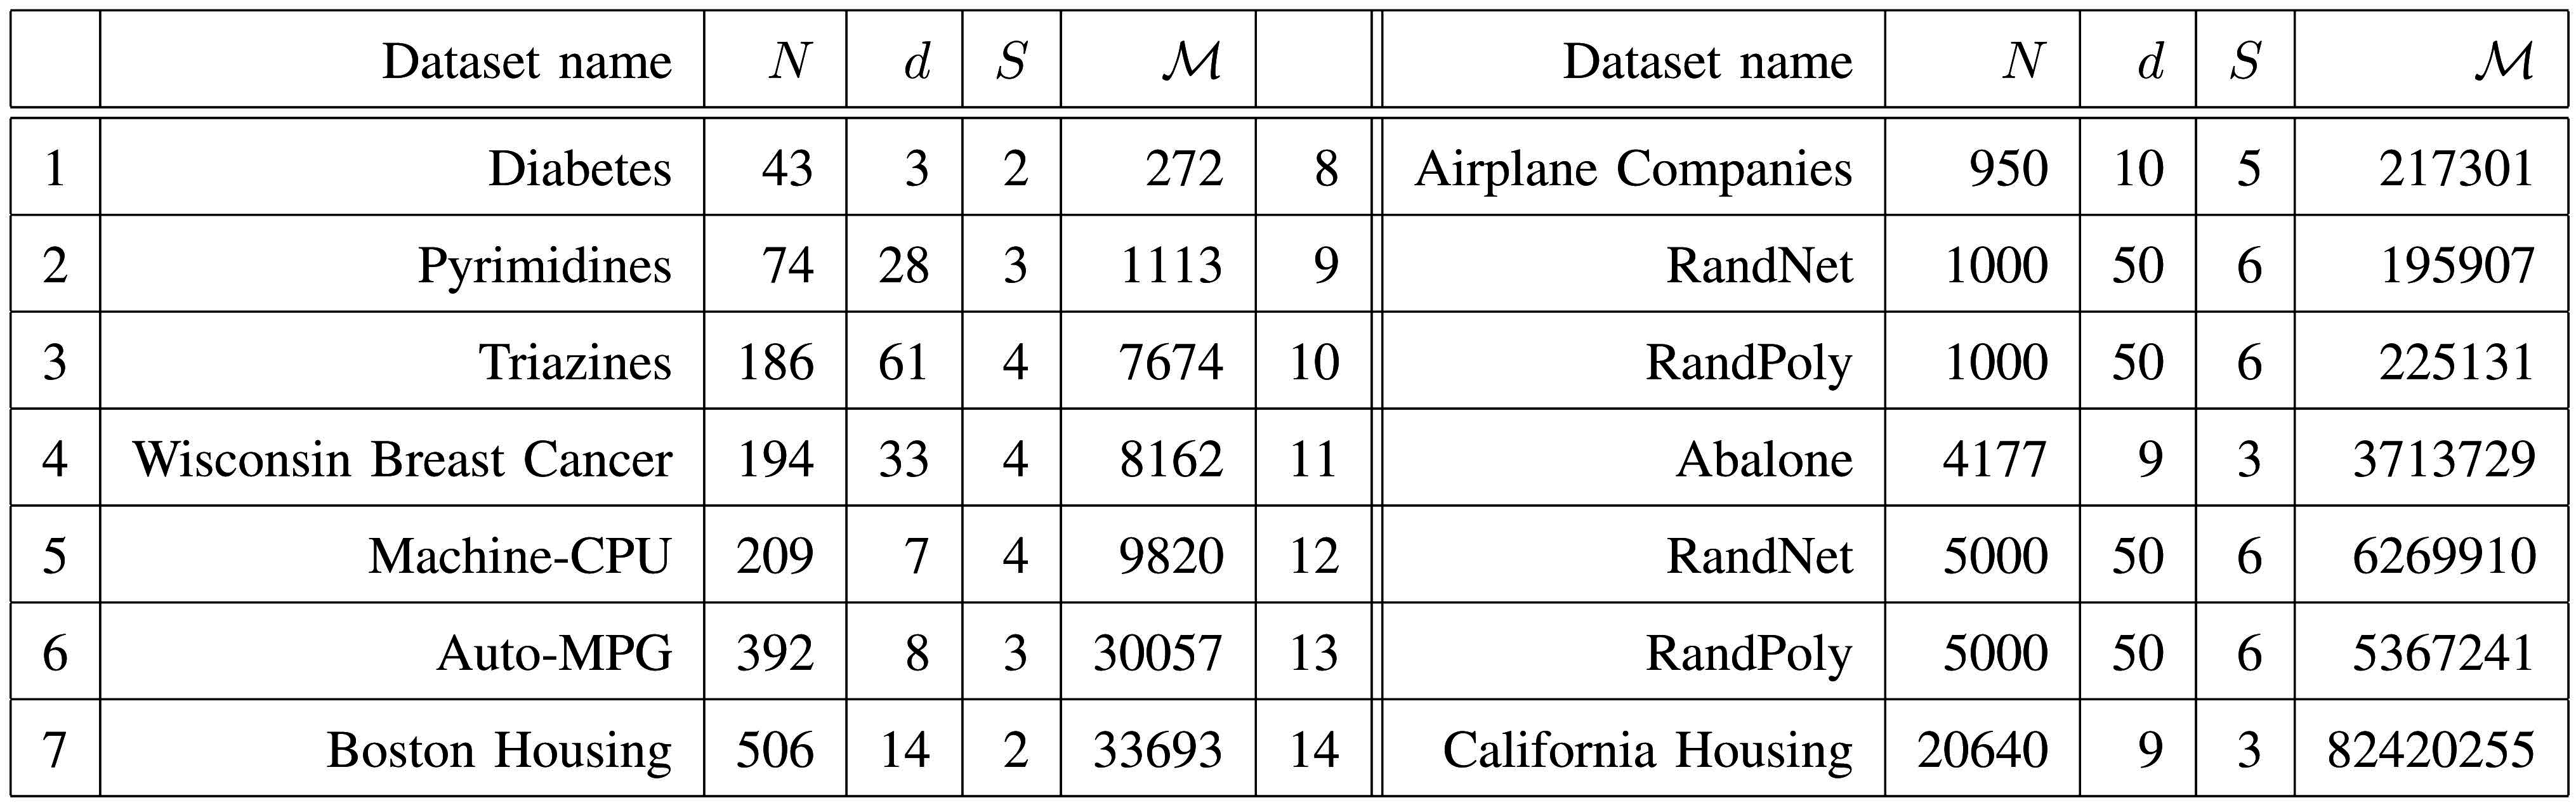
\includegraphics[width=\textwidth]{datasets}
    \caption{$N$ is the size of the data set. $d$ is the number of attributes. $S$ is the number of classes. $M$ is the average total number of pairwise relations per fold of the training set.}\label{tab:res_db}
    \end{table}
\end{frame}

%\begin{frame}{Ranking Experiments}{Evaluation Procedure}
%    \begin{itemize}
%    \item For each data set, 80 percent of the examples were used for training and the remaining 20 percent were used for testing.
%    \item The results are shown for a fivefold cross validation experiment.
%    \end{itemize}
%\end{frame}

\begin{frame}{Ranking Experiments}{Results}
    \onslide{\footnotesize The results are shown for a five fold cross-validation experiment. The symbol $\star$ indicates that the particular method either crashed due to limited memory requirements or took a very large amount of time.}
    \begin{table}
    \centering
    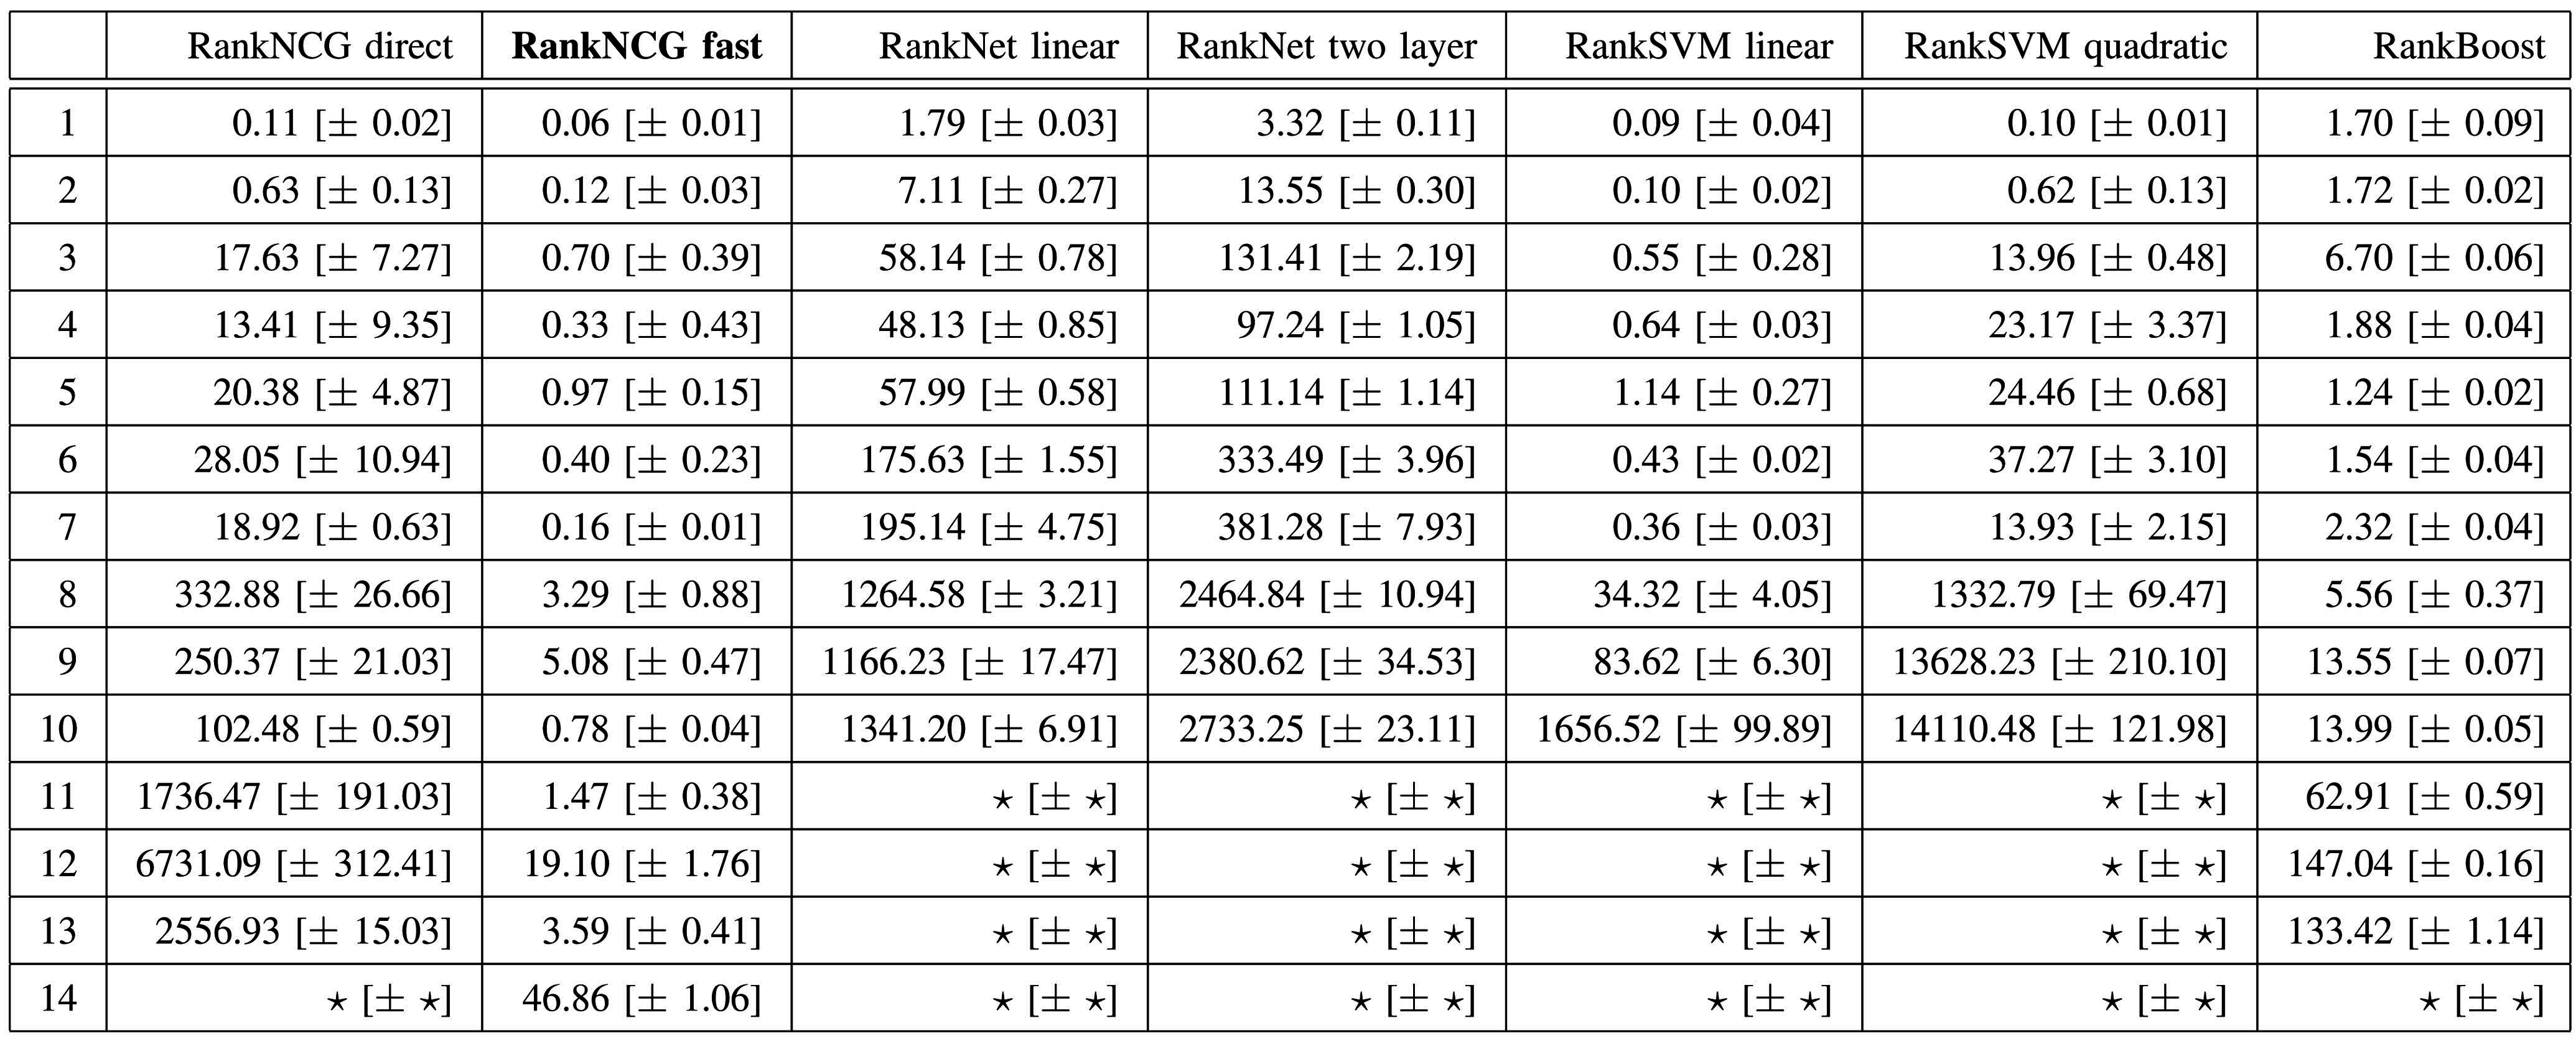
\includegraphics[width=\textwidth]{results-time-over-db}
    \caption{The Mean Training Time and Standard Deviation in Seconds for the Various Methods and All the Data Sets Shown in Table \ref{tab:res_db}}\label{tab:res_time_over_db}
    \end{table}
\end{frame}

\begin{frame}{Ranking Experiments}{Results}
    \onslide{\footnotesize The results are shown for a five fold cross-validation experiment. The symbol $\star$ indicates that the particular method either crashed due to limited memory requirements or took a very large amount of time.}
    \begin{table}
    \centering
    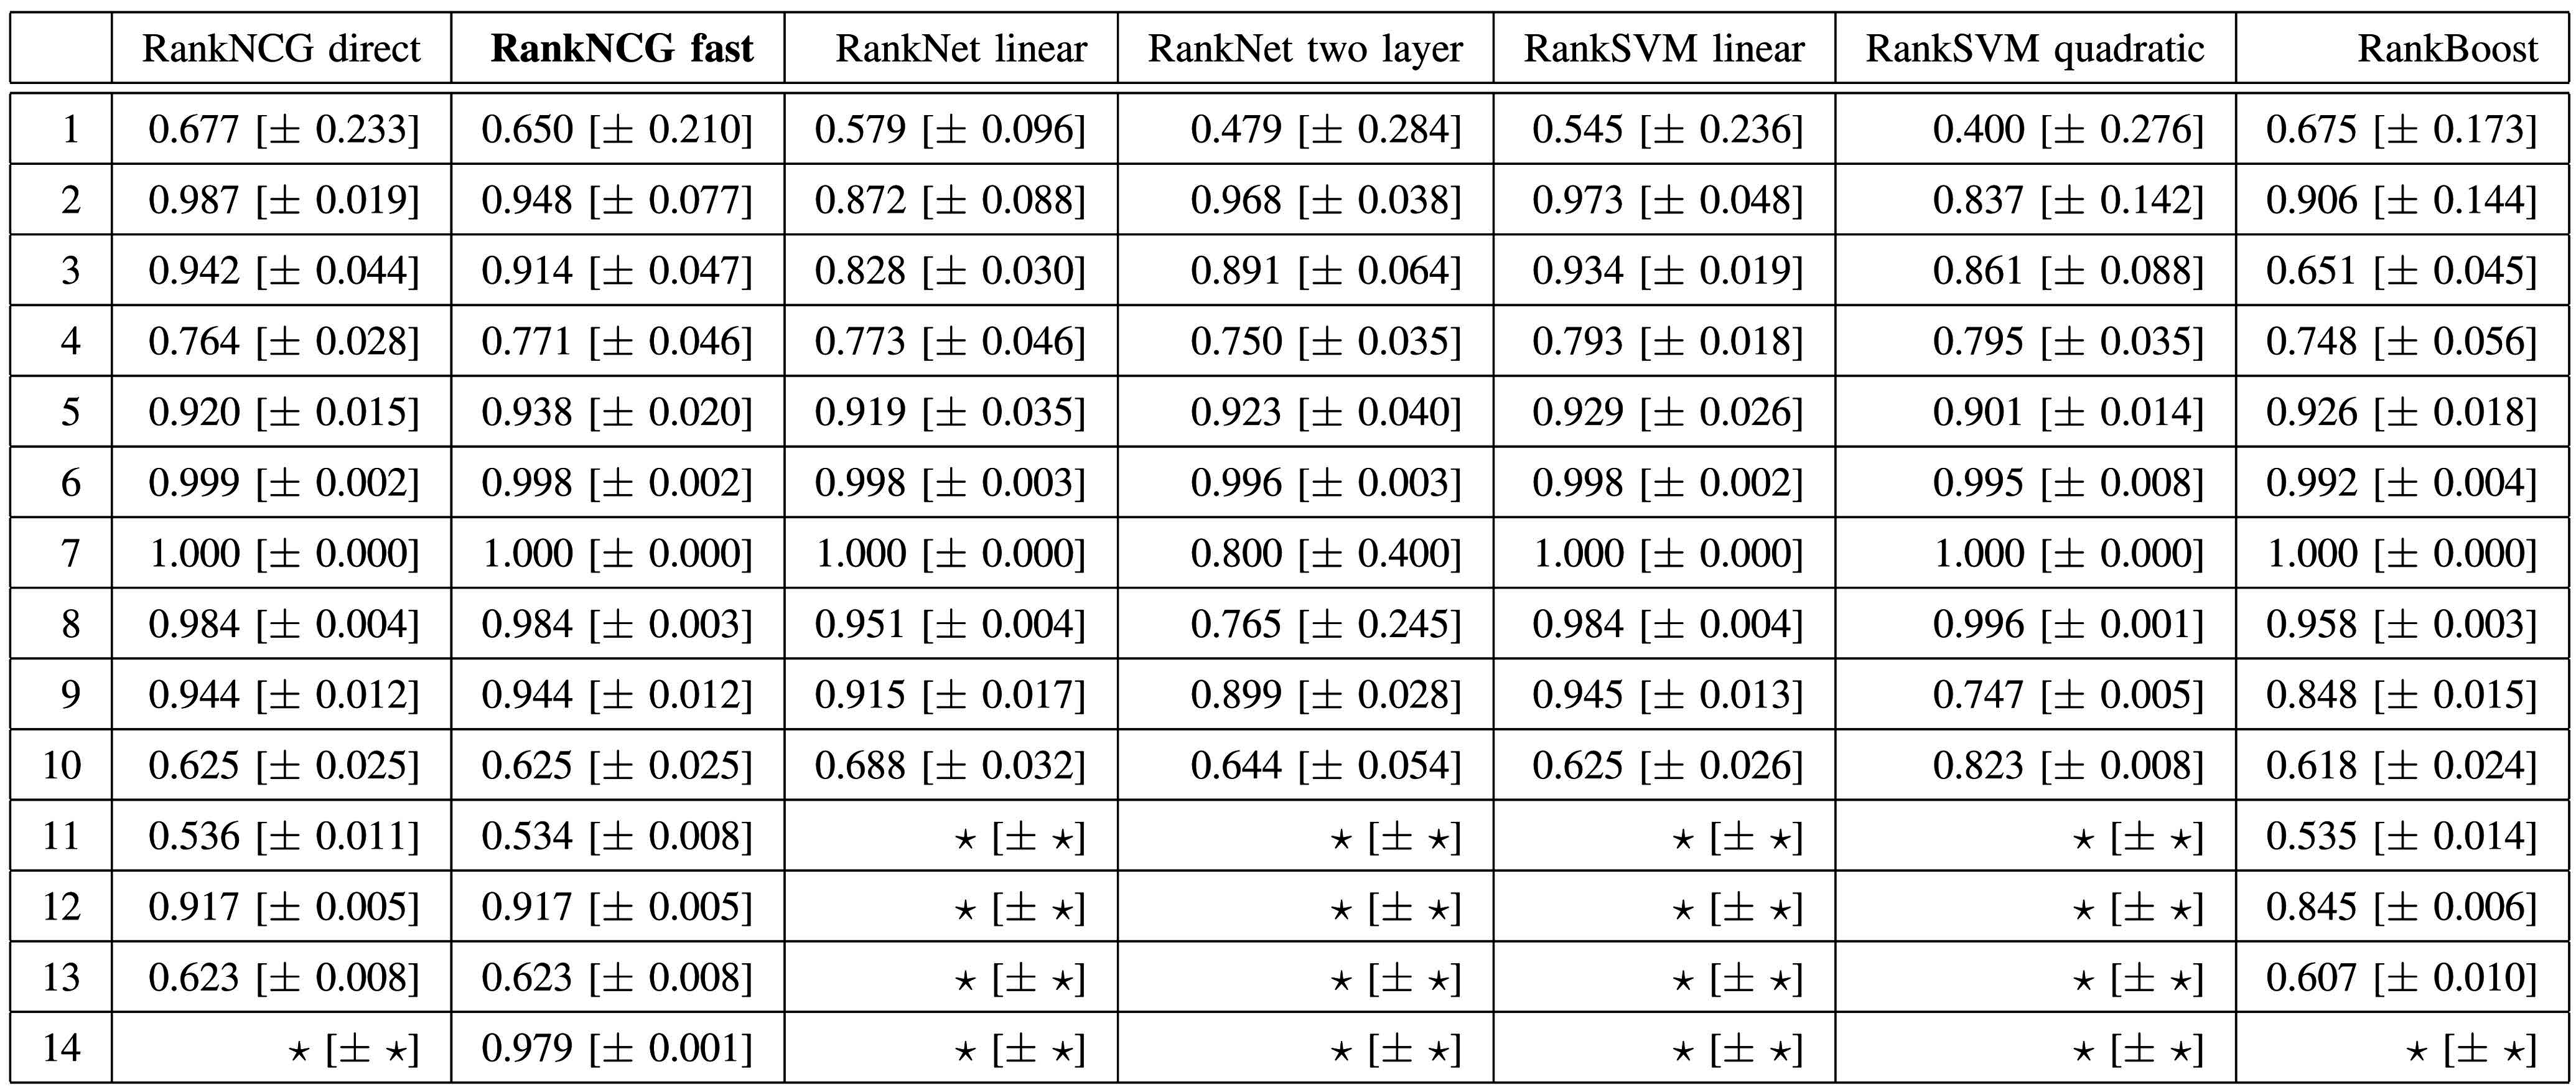
\includegraphics[width=\textwidth]{results-wmw-stat-over-db}
    \caption{The Corresponding Generalized WMW Statistic and the Standard Deviation on the Test Set for the Results Shown in Table \ref{tab:res_time_over_db}}\label{tab:res_wmw_stat_over_db}
    \end{table}
\end{frame}

\section{Conclusion}
\begin{frame}{Conclusion}
    \begin{itemize}
    \item This paper, presented an approximate ranking algorithm that directly maximizes (a regularized lower bound on) the generalized Wilcoxon-Mann-Whitney statistic.
    \item The algorithm was made computationally tractable using a novel fast summation method for calculating a weighted sum of erfc functions.
    \item Experimental results demonstrate that despite the order of magnitude speedup, the accuracy was almost identical to exact method and other algorithms proposed in literature.
    \end{itemize}
\end{frame}

\begin{frame}{}
    \begin{center}
    \vspace{5em}
    {\fontsize{20}{50}\selectfont Thank You!}
    \end{center}
    \begin{tikzpicture}[remember picture,overlay]
      \node[anchor=south west,inner sep=0pt] at (7cm,-3cm) {
         
\includegraphics[width=.2\textwidth]{Question_mark_robot}
      };
    \end{tikzpicture}
\end{frame}

\section{References}
\begin{frame}{References}
    \nocite{*}
    {\scriptsize
    \bibliographystyle{IEEEtran}
    \bibliography{reference}
    }
\end{frame}

\appendix

\end{document}